% ZÁVĚREČNÁ STUDIJNÍ PRÁCE – Jakub Netolický – prazmas

\documentclass[12pt, a4paper,
%oneside,
]{report}

% --- čištění zbytků z původní šablony ---
\AtBeginDocument{%
  \immediate\write16{(cleaning stray figureversions output...)}%
  \thispagestyle{empty}%
  \let\superiorSup\relax
  \let\textOsF\relax
  \let\textTOsF\relax
  \let\liningLF\relax
  \let\liningTLF\relax
  \let\tabularTab\relax
  \let\proportionalProp\relax
  \let\tabularmath\relax
  \let\proportionalmath\relax
  \let\fontspechyperref\relax
}

% ===================== PROMĚNNÉ =====================

\newcommand\obor{INFORMAČNÍ TECHNOLOGIE}
\newcommand\kodOboru{18-20-M/01}
\newcommand\zamereni{se zaměřením na počítačové sítě a programování}
\newcommand\skola{Střední škola průmyslová a umělecká, Opava}
\newcommand\trida{IT4}
\newcommand\jmenoAutora{Jakub Netolický}
\newcommand\skolniRok{2025/26}
\newcommand\datumOdevzdani{1. 1. 2026} % uprav podle reálného data
\newcommand\nazevPrace{Desktopová aplikace pro přehrávání a editování hudby pro tanec}

\title{\nazevPrace}
\author{\jmenoAutora}
\date{\datumOdevzdani}

% ===================== BALÍČKY =====================

\usepackage[top=2.5cm, bottom=2.5cm, left=3.5cm, right=1.5cm]{geometry}
\flushbottom                    % <-- PŘIDEJ TOHLE
\makeatletter
\makeatother                    
\usepackage[czech]{babel}
\hyphenation{apli-ka-ce}
\hyphenation{pra-zmas}
\clubpenalty=10000
\widowpenalty=10000
\tolerance=2000
\finalhyphendemerits=5000
\usepackage[utf8]{inputenc}
\usepackage[T1]{fontenc}
\usepackage{cmap}
\usepackage{graphicx}
\usepackage{subcaption}
\usepackage{hyperref}
\linespread{1.25}
\setlength{\parskip}{0.5em}

\usepackage[pagestyles]{titlesec}
\titleformat{\chapter}[block]{\scshape\bfseries\LARGE}{\thechapter}{10pt}{\vspace{0pt}}[\vspace{-22pt}]
\titleformat{\section}[block]{\scshape\bfseries\Large}{\thesection}{10pt}{\vspace{0pt}}
\titleformat{\subsection}[block]{\bfseries\large}{\thesubsection}{10pt}{\vspace{0pt}}

\usepackage{tocloft}
\setlength{\cftbeforechapskip}{0pt}
\setlength{\cftbeforesecskip}{0pt}
\setcounter{secnumdepth}{3}
\setcounter{tocdepth}{3}

\usepackage{fancyhdr}
\pagestyle{fancy}
\renewcommand{\headrulewidth}{0.025pt}

\usepackage{booktabs}
\usepackage{url}
\usepackage{pdfpages}
\usepackage{upgreek}
\usepackage{amsmath}
\usepackage{amsfonts}
\usepackage{esint}
\usepackage{mathrsfs}
\usepackage{helvet}
\usepackage{mathptmx}

\makeatletter
\@namedef{ver@figureversions.sty}{9999/99/99}
\newcommand{\DeclareFigureVersion}[2]{}
\newcommand{\figureversion}[1]{}
\makeatother

\makeatletter
\providecommand{\superiorSup}{}
\providecommand{\textOsF}{}
\providecommand{\textTOsF}{}
\providecommand{\liningLF}{}
\providecommand{\liningTLF}{}
\providecommand{\tabularTab}{}
\providecommand{\proportionalProp}{}
\providecommand{\tabularmath}{}
\providecommand{\proportionalmath}{}
\makeatother

\usepackage{listings}
\usepackage{xcolor}
\renewcommand{\lstlistingname}{Kód}
\renewcommand{\lstlistlistingname}{Seznam programových kódů}

\let\cleardoublepage\clearpage
\makeatletter
\renewcommand{\@openrightfalse}{\let\cleardoublepage\clearpage}
\makeatother

% ===================== DOKUMENT =====================

\begin{document}

\pagestyle{empty}
\pagenumbering{Roman}
\cleardoublepage

% ---------- TITULNÍ STRÁNKA ----------

{\fontfamily{phv}\selectfont

\begin{figure}[h]
  \centering
  
\includegraphics[width=0.6\linewidth]{image/logo-skoly.png}
\end{figure}

{\bfseries
\begin{center}
  \vspace{0.025 \textheight}
  \LARGE{ZÁVĚREČNÁ STUDIJNÍ PRÁCE}\\
  \large{dokumentace}\\
  \vspace{0.075 \textheight}
  \LARGE {\nazevPrace}\\[1.5em]
  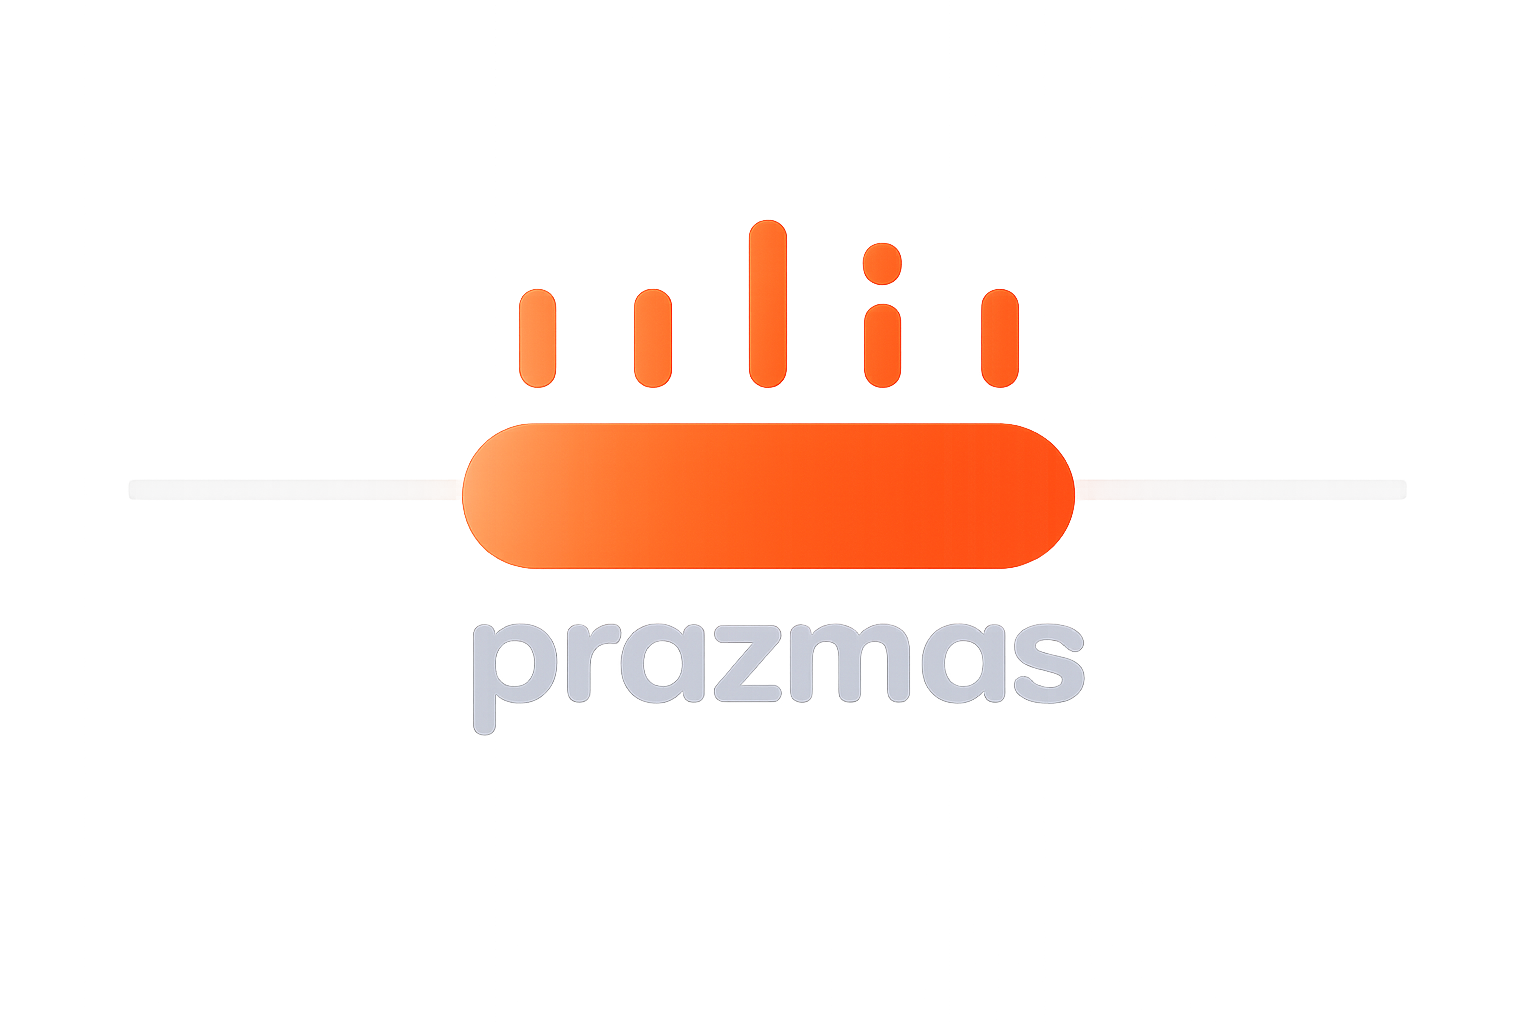
\includegraphics[width=0.45\linewidth]{image/prazmas-logo.png}\\[0.5em]
\end{center}
}

\vspace{0.02 \textheight}

\begin{table}[h!]
\begin{tabular}{ll}
\textbf{Autor:} & \jmenoAutora\\
\textbf{Obor:} & \kodOboru\ \obor\\
\textbf{} & \zamereni\\
\textbf{Třída:} & \trida\\
\textbf{Školní rok:} & \skolniRok\\
\end{tabular}
\end{table}
}

\cleardoublepage

% ---------- PODĚKOVÁNÍ A PROHLÁŠENÍ ----------

\noindent{\large{\bfseries{Poděkování}\\}}
\noindent Prostor k poděkování (například mně, testerům aplikace atd.).

\vspace*{0.7\textheight}

\noindent{\large{\bfseries{Prohlášení}\\}}
\noindent{Prohlašuji, že jsem závěrečnou práci vypracoval samostatně a uvedl veškeré použité informační zdroje.}\\[0.5em]
\noindent{Souhlasím, aby tato studijní práce byla použita k výukovým a prezentačním účelům na Střední průmyslové a umělecké škole v Opavě, Praskova 399/8.}

\vfill
\noindent{V Opavě \datumOdevzdani\\}
\noindent
\begin{minipage}{\linewidth}
  \hspace{9.5cm}
  \begin{tabular}{@{}p{6cm}@{}}
    \dotfill \\
    Podpis autora
  \end{tabular}
\end{minipage}

\cleardoublepage

% ---------- ABSTRAKT CZ/EN ----------

\noindent{\Large{\bfseries{Anotace}\\}}
\noindent
Výsledkem projektu je desktopová aplikace \textit{prazmas} pro skládání tréninkových hudebních mixů určených zejména pro párové tance. Aplikace umožňuje import hudebních skladeb, jejich zobrazení ve formě waveformu a rozdělení na jednotlivé úseky (buňky), které lze libovolně řadit do timeline. Uživatel může měnit tempo jednotlivých úseků, nastavovat fade-in a fade-out, hlasitost nebo jednoduchý echo efekt a vytvářet tak plynulé tréninkové sestavy. Součástí je také automatické generování „practice“ mixů – aplikace pro daný tanec vyhledá vhodné skladby v lokální knihovně a pomocí jednoduché AI ověří, zda hudba stylově odpovídá. Výstupem je mixdown ve formátu WAV, případně MP3/FLAC, použitelný při výuce i domácím tréninku; všechny vytvořené mixy lze exportovat pro další použití.

\vspace{18pt}
\noindent{\large{\bfseries{Klíčová slova}}}\\
\noindent prazmas, hudební aplikace, trénink tanců, PyQt6, audio, FFmpeg

\vspace{18pt}

\noindent{\Large{\bfseries{Abstract}\\}}
\noindent
The project results in a desktop application called \textit{prazmas} designed for creating practice music mixes, primarily for ballroom and latin dances. The application imports audio tracks, displays their waveforms and lets the user split them into segments that can be arranged on a timeline. Each segment supports tempo changes, gain adjustments, fade-in and fade-out or a simple echo effect to build smooth training routines. The application can also automatically generate practice mixes by selecting suitable songs for a given dance from the local library and validating their style using a lightweight AI component. The final arrangement can be exported as a WAV file or encoded to MP3/FLAC for everyday practice; every created mix can be saved for later use.

\vspace{18pt}
\noindent{\large{\bfseries{Keywords}}}\\
\noindent prazmas, music practice tool, ballroom dance, PyQt6, audio, FFmpeg

\clearpage

% ---------- OBSAH ----------

\tableofcontents
\pagenumbering{arabic}
\setcounter{page}{1}

% ====================================================
%                    KAPITOLY
% ====================================================

\chapter*{Úvod}
\addcontentsline{toc}{chapter}{Úvod}

Trénink soutěžních tanců je dnes často organizován formou takzvaných \emph{practice} bloků, které napodobují průběh skutečné soutěže – pouští se celé skladby jednotlivých tanců, mezi nimi jsou jen krátké pauzy v řádu desítek sekund. Na běžných trénincích se proto střídá hudba z YouTube, stažené písničky a hotové prakticy, které jsou ale pevně dané a snadno se začnou opakovat.

Používané nástroje jsou většinou obyčejné přehrávače jako Windows Media Player nebo VLC. Ty sice zvládnou základní přehrávání, ale neumožňují rychlou změnu tempa, jednoduché vytváření loopů ani skládání více skladeb do jednoho uceleného practice mixu, nebo jiných složených celků. Jakmile chce trenér něco upravit – zkrátit skladbu, změnit tempo nebo přehodit pořadí tanců – musí ručně manipulovat s playlisty nebo přeskakovat mezi okny, což zdržuje průběh tréninku a omezuje možnosti práce s hudbou.

Cílem této práce bylo proto vytvořit jednoduchou, ale specializovanou desktopovou aplikaci \textit{prazmas}, která umožní pohodlnou práci s hudbou přímo během tréninku. Aplikace má nabídnout přehledný editor s časovou osou, podporu loopů, rychlou změnu tempa a možnost náhodného generování practice mixů tak, aby se stále neopakovaly stejné sestavy. Součástí je také vlastní AI modul pro rozpoznávání tanečního stylu jednotlivých skladeb, který pomáhá kontrolovat, že zvolená hudba odpovídá požadovanému tanci.

\chapter{Motivace a cíle projektu}

\section{Proč vznikla aplikace \textit{prazmas}}

Z vlastní zkušenosti z tréninků vyplynulo, že současné řešení práce s hudbou je spíše provizorní. Během practice se střídají skladby pouštěné z YouTube a lokálně uložené písničky nebo celé dříve připravené prakticy, které se postupem času opakují. Možnosti, jak s hudbou aktivně pracovat přímo na tréninku, jsou omezené: chybí jednoduché vytváření loopů, plynulá změna tempa i rychlá úprava pořadí tanců bez složitého editování playlistů.

Vyzkoušené nástroje, jako jsou běžné systémové přehrávače (například Windows Media Player nebo VLC), případně univerzální programy pro přehrávání hudby, fungují dobře jako klasické přehrávače, ale nenabízejí funkce potřebné pro taneční tréninky. Neumožňují náhodné skládání nových prakticů z knihovny skladeb, neumějí pracovat s tanečními styly ani neumí jednoduše změnit tempo tak, aby se daly skladby přizpůsobit konkrétnímu tréninkovému plánu. Z tohoto důvodu se ukázalo jako vhodné navrhnout vlastní nástroj zaměřený přímo na potřeby trenérů a tanečníků.

Při návrhu ideálního řešení byl kladen důraz na to, aby bylo možné připravit nebo spustit practice v několika málo krocích. Trenér by měl mít k dispozici jedno hlavní okno s knihovnou skladeb, editorem timeline a viditelnými ovládacími prvky pro tempo, hlasitost a loop. Původní myšlenkou bylo vytvořit webovou aplikaci, ale s ohledem na potřebu spolehlivého přehrávání zvuku, nižší latence a nezávislosti na internetovém připojení padla volba na offline desktopovou aplikaci pro Windows, kterou lze v~případě potřeby buildnout i pro Linux.

\newpage
\section{Cíle práce}

Hlavním cílem projektu je navrhnout a implementovat desktopovou aplikaci \textit{prazmas}, která zjednoduší přípravu a přehrávání tréninkových hudebních mixů. Z tohoto obecného cíle vyplývají dílčí cíle:

\begin{itemize}
  \item umožnit uživateli skládat practice mixy z náhodných skladeb v lokální knihovně, včetně jednoduché tvorby loopů a skládání více písniček do sebe;
  \item implementovat rychlou a intuitivní změnu tempa jednotlivých úseků, aby bylo možné přizpůsobit hudbu požadovanému rytmu bez nutnosti složitého offline střihu;
  \item zavést systém náhodného generování practice mixů, který na základě parametrů (například délka jednoho tance, délka pauzy, volba standardních nebo latinských tanců) automaticky vybere vhodné skladby z knihovny a předejde opakování stále stejných sestav;
  \item integrovat vlastní vytrénovaný AI modul, který pro každou skladbu určí procentuální zastoupení jednotlivých tanečních stylů a zobrazí přehlednou tabulku pravděpodobností tak, aby bylo možné ověřit, zda skladba odpovídá zamýšlenému tanci;
  \item umožnit export výsledného mixu do běžných audio formátů (WAV, případně MP3 nebo FLAC), aby bylo možné vytvořené prakticy snadno používat na různých zařízeních i mimo samotnou aplikaci.
\end{itemize}

Aplikace je v první řadě určena pro trenéry a tanečníky, kteří potřebují mít pod kontrolou hudební doprovod na trénincích, ale může posloužit i dalším uživatelům pro jednoduchou editaci a skládání hudby bez nutnosti učit se práci s komplexním zvukovým editorem.

\chapter{Použité technologie}

Tato kapitola popisuje technologie a knihovny, na kterých je aplikace \textit{prazmas} postavena. Cílem je ukázat, jaké nástroje byly pro vývoj zvoleny, jakou roli v aplikaci hrají a jak spolu jednotlivé části souvisejí.

\section{Programovací jazyk Python a PyQt6}

Jako hlavní programovací jazyk byl zvolen Python. Aplikace \textit{prazmas} je vyvíjena a provozována v prostředí Python~3.12.10 na 64bitové platformě Windows, spuštěné v odděleném virtuálním prostředí projektu. Tato verze poskytuje moderní jazykové konstrukce, bohatý ekosystém knihoven pro práci se zvukem, GUI i strojové učení a zároveň je kompatibilní s použitými externími moduly.

\begin{figure}[h!]
  \centering
  
\includegraphics[width=0.5\textwidth]{image/pyqt6-logo.png}
  \caption{knihovna PyQt6.}
  \label{fig:pyqt6-logo.png}
\end{figure}

Grafické uživatelské rozhraní je postaveno na knihovně PyQt6, což je vazba na toolkit Qt určený pro tvorbu multiplatformních GUI aplikací. PyQt6 poskytuje širokou škálu widgetů, správu layoutů, práci s událostmi a časovači, což je v \textit{prazmas} využito například pro vykreslování waveformu, správu časové osy a ovládání přehrávání. Hlavní okno aplikace je implementováno ve třídě \texttt{MainWindow}, která dědí od \texttt{QMainWindow} a vytváří kompletní rozložení UI včetně knihovny skladeb, timeline, editoru buněk a ovládacích prvků přehrávání.

\newpage
\section{Práce se zvukem: pydub, FFmpeg a vlastní audio vrstva}

Základní zpracování zvuku, jako je načítání audio souborů, dělení na úseky, aplikace efektů a renderování výsledného mixu, je řešeno pomocí knihovny \texttt{pydub}. Pydub poskytuje vysokou úroveň abstrakce nad audiem – umožňuje jednoduše číst soubory přes FFmpeg, skládat je za sebe, překrývat, aplikovat fade-in a fade-out nebo měnit hlasitost. V aplikaci \textit{prazmas} se pydub používá například při generování practice mixů a při exportu výsledného aranžmá do dočasného WAV souboru.

Pro samotnou konverzi formátů a dekódování vstupních souborů je využit nástroj FFmpeg, který pydub interně používá. Aby aplikace fungovala, musí být FFmpeg dostupný v systémové cestě (PATH); při chybějící instalaci aplikace zobrazí uživateli chybové hlášení a vysvětlí, že bez FFmpegu není možné provádět mixdown.

Nízkou úroveň přehrávání řeší modul \texttt{audio.player}, kde třída \texttt{AudioPlayer} poskytuje rozhraní pro načtení audio souboru, spuštění přehrávání, pauzu, zastavení, skok na požadovanou pozici a volitelné nastavení loopu. \texttt{AudioPlayer} je úzce provázán s \texttt{MainWindow}, které jej používá jako backend pro přehrávání jak originální skladby, tak vygenerovaného mixdownu. Pro úpravy tempa se využívá funkce \texttt{rendervariant} v modulu \texttt{audio.processing}, která dokáže z původního souboru vytvořit nový WAV soubor s upravenou rychlostí.

\section{Grafické komponenty: timeline a editor buněk}

Aplikace \textit{prazmas} obsahuje dvě klíčové grafické komponenty pro práci s aranžmá: časovou osu (\texttt{TimelineWidget}) a editor buněk (\texttt{TrackEditorWidget}). Obě komponenty jsou implementovány jako vlastní widgety nad třídami Qt a umožňují detailní vizuální manipulaci s hudebním materiálem.

\subsection{TimelineWidget}

Třída \texttt{TimelineWidget} se stará o zobrazení průběhu celého aranžmá v čase. 
Zobrazuje horizontální osu s časovým měřítkem, waveform výsledného mixu a polohu přehrávací hlavy. 
Uživatel může kliknutím na časovou osu měnit pozici přehrávání, 
případně nastavovat oblast loopu pomocí dvou značek (A/B), jak je vidět na obr.~\ref{fig:timeline-loop}. 
Widget také emituje signály \texttt{seekRequested}, \texttt{loopAChanged}, \texttt{loopBChanged} 
a \texttt{clearLoopRequested}, na které \texttt{MainWindow} reaguje aktualizací stavu přehrávače a editoru.

\begin{figure}[h!]
  \centering
  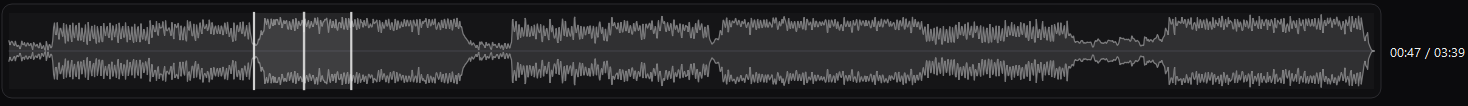
\includegraphics[width=0.85\textwidth]{image/timeline-loop.png}
  \caption{Timeline s aktivním A/B loopem (červené značky), přehrávací hlavou (žlutá čára) 
  a zoomovaným měřítkem pro přesné nastavení.}
  \label{fig:timeline-loop}
\end{figure}

\subsection{TrackEditorWidget a struktura Cell}

Základem pro skládání hudby je třída \texttt{TrackEditorWidget}, která zobrazuje jednotlivé úseky (buňky) na více „lanech“ v horizontálním čase. Každá buňka je reprezentována datovou strukturou \texttt{Cell}, definovanou jako dataclass se základními parametry: číslo lane, offset v milisekundách, délka, cesta k souboru, titulek, waveform, přirozená délka v původním tempu, aktuální tempo, fade-in a fade-out, zisk v decibelech a parametry echo efektu.

\texttt{TrackEditorWidget} umožňuje buňky horizontálně a vertikálně posouvat, 
kopírovat a dělit. Pomocí kontextového menu (obr.~\ref{fig:editor-menu}) lze na vybranou 
buňku aplikovat efekty (gain, fade-in, fade-out a echo), nebo buňku rozdělit na dvě části 
v zadaném čase.
 Widget také podporuje přetahování souborů z operačního systému a položek z knihovny skladeb – při dropu vytvoří novou buňku s odpovídajícím waveformem a délkou. Při každé změně aranžmá vysílá signál \texttt{arrangementChanged}, na který hlavní okno reaguje přepočtem celkové délky a přípravou mixdownu.

 \begin{figure}[h!]
  \centering
  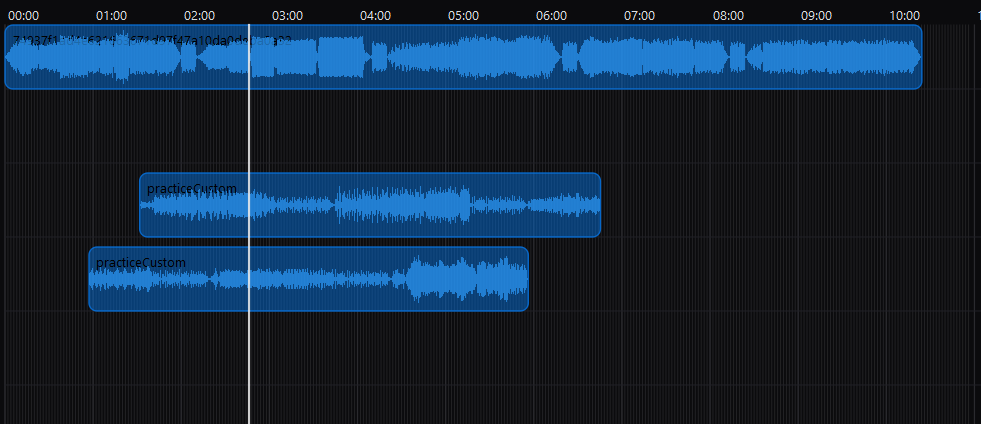
\includegraphics[width=0.7\textwidth]{image/editor-bunka-menu.png}
  \caption{Kontextové menu buňky s možnostmi ``Cut at playhead'', ``Echo effect'', 
  ``Fade-in/out'' a nastavením gain.}
  \label{fig:editor-menu}
\end{figure}

\section{AI modul pro rozpoznávání tanečních stylů}

Součástí aplikace je vlastní AI modul, který pro každou skladbu odhaduje pravděpodobnost příslušnosti k jednotlivým tanečním stylům. Tato funkcionalita je implementována v balíčku \texttt{ml}.

Modul \texttt{features.py} obsahuje funkce pro extrakci příznaků ze zvuku – například spektrální vlastnosti, rytmické rysy a další statistiky, které se dají využít pro strojové učení. Tyto příznaky jsou využity při trénování a inferenci modelu.

Trénování modelu je řešeno v souboru \texttt{train.py}, kde se na základě anotovaných zvukových ukázek jednotlivých tanců vytvoří klasifikátor rozlišující jednotlivé styly. Seznam podporovaných štítků a jejich indexů je udržován v modulu \texttt{labels\_index.py}, který zajišťuje konzistenci mezi tréninkem a inferencí. Pro automatické labelování dat může sloužit pomocný skript \texttt{auto\_label.py}.

V samotné aplikaci je AI modul zapouzdřen ve třídě \texttt{DanceAI} v souboru \texttt{infer.py}. Tato třída poskytuje metody \texttt{predict} a \texttt{predict\_proba\_all}, které na základě vstupního audio souboru vrátí jednak nejpravděpodobnější taneční styl, jednak rozložení pravděpodobností přes všechny styly. Výsledek se v UI zobrazuje jako tabulka procent (obr.~\ref{fig:ai-analyza}), 
která dohromady tvoří 100\,\%, doplněná odhadem BPM. Uživatel tak může okamžitě zkontrolovat, zda skladba odpovídá například sambě, chachě, rumbě nebo standardním tancům.

\begin{figure}[h!]
  \centering
  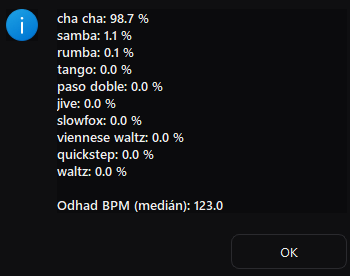
\includegraphics[width=0.6\textwidth]{image/ai-analyza.png}
  \caption{AI analýza skladby: Cha-Cha 98,7\,\%, Samba 1,1\,\%, BPM 123.}
  \label{fig:ai-analyza}
\end{figure}

\section{Knihovna skladeb a správa souborů}

Hudební soubory, se kterými aplikace pracuje, jsou organizovány pomocí modulu \texttt{library.manager}. Tento modul zajišťuje uložení informací o skladbách, jako je název, cesta k souboru, délka a případně další metadata. Hlavní okno s knihovnou využívá třídu \texttt{Library}, která nabízí metody pro přidání nových souborů, získání cesty ke skladbě, výpis všech skladeb nebo práci s oblíbenými položkami.

Pro zobrazení knihovny v UI slouží specializovaný widget \texttt{TrackListWidget} ze souboru \texttt{track\_list.py}. Ten rozšiřuje standardní \texttt{QListWidget} o podporu kontextového menu (například označení skladby jako oblíbené, spuštění přehrávání nebo vyvolání AI analýzy). Kromě toho umožňuje přetahování skladeb do editoru buněk, kde se z nich okamžitě vytvoří nové buňky s waveformem.

Aplikace také podporuje ukládání a obnovu stavu knihovny, včetně jednoduchého systému oblíbených skladeb. Pokud databáze knihovny některé soubory nenajde, nabízí funkce pro „opravu“ a „relink“ – uživatel může zvolit novou cestu k souborům a knihovna se podle toho aktualizuje.

\section{Vlastní vzhled a ovládací prvky}

\begin{figure}[h!]
  \centering
  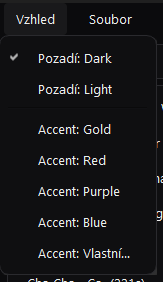
\includegraphics[width=0.5\textwidth]{image/theme-dialog.png}
  \caption{Dialog výběru barevného motivu aplikace.}
  \label{fig:theme-dialog.png}
\end{figure}

Pro sjednocení vzhledu aplikace a možnost přepínání motivů je vytvořen modul \texttt{ui.theme}. Ten definuje třídu \texttt{Theme} s parametry jako barevný režim (světlý/tmavý) a akcentová barva a rovněž generuje odpovídající Qt Style Sheet (QSS). Hlavní okno umí téma načíst, uložit do souboru a aplikovat na celou aplikaci; zároveň obsahuje menu pro přepínání motivu a výběr akcentové barvy. Speciální widgety jako \texttt{TimelineWidget} a \texttt{TrackEditorWidget} dokáží motiv převzít a podle něj upravit barvy gridu, waveformu a buněk.


Mezi vlastní ovládací prvky patří také widget \texttt{PlayPauseButton}, který zabalí logiku přehrávání do jednoho přepínacího tlačítka s ikonou a stavem. V kombinaci s \texttt{WinMediaKeyFilter} je možné reagovat i na systémové multimediální klávesy, takže uživatel může pauzovat a spouštět přehrávání přímo z klávesnice nebo z ovladače připojeného k počítači.

Tyto vlastní komponenty doplňují standardní sadu widgetů Qt a umožňují, aby aplikace působila vizuálně konzistentně, byla snadno ovladatelná a zároveň nabízela funkce, které v běžných přehrávačích hudby chybí.

Další oblastí, na kterou byl kladen důraz, je pohodlné ovládání přehrávání i v situaci, kdy je aplikace minimalizovaná nebo běží na pozadí. Kromě klasických ovládacích prvků v hlavním okně podporuje \textit{prazmas} také reakce na multimediální klávesy systému a tlačítka na bezdrátových sluchátkách.

V praxi to znamená, že uživatel může spouštět a zastavovat přehrávání i pomocí tlačítka Play/Pause na sluchátkách (například typu true‑wireless), případně pomocí dedikovaných kláves na klávesnici nebo dálkovém ovladači. Tato funkcionalita je realizována kombinací vlastního přepínacího tlačítka \texttt{PlayPauseButton} a modulu, který zachytává systémové multimediální události a předává je do hlavního okna aplikace.

\chapter{Návrh a postup realizace}

\section{Vývoj uživatelského rozhraní a funkcí}

Vývoj aplikace \textit{prazmas} probíhal iterativně, kdy se postupným přidáváním nových funkcí měnilo jak rozložení uživatelského rozhraní, tak i vnitřní architektura. Úplně první funkční verze byla v podstatě jednoduchý přehrávač: obsahovala pouze časovou osu, ovládací tlačítka \texttt{Open}, \texttt{Previous}, \texttt{Play/Pause}, \texttt{Next}, posuvník hlasitosti a ovládání tempa. Timeline v této fázi ještě nebyla vizuálně propracovaná, ale umožňovala základní orientaci v průběhu skladby a ruční posun přehrávací hlavy.

Dalším krokem bylo přidání knihovny skladeb, která se postupně stala jednou z hlavních částí rozhraní. Přidáním knihovny se výrazně změnil typický pracovní postup: uživatel už nemusel jednotlivé soubory otevírat ručně z diskového dialogu, ale měl přehledný seznam skladeb s možností vyhledávání a filtrování. V praxi se ukázalo, že při mazání nebo přesunu souborů může v databázi knihovny zůstat záznam na neexistující cestu, a proto byla doplněna funkce „Opravit“, která knihovnu zkontroluje a umožní chybějící soubory buď znovu nalinkovat, nebo z databáze odstranit.

Po stabilizaci knihovny byla aplikace rozšířena o režim \emph{Autoplay}. Ten zajišťuje, že po skončení jedné skladby automaticky začne hrát další položka podle aktuálního filtru v knihovně. Trenér tak nemusí při practice neustále ručně přepínat skladby a může se soustředit na práci s tanečníky. Následovala implementace skládání practice bloků: uživatel získal možnost zvolit parametry jako typ tance (standardní či latinské), délku jednotlivých skladeb a délku pauz a aplikace na jejich základě náhodně vybere vhodné skladby z knihovny a vytvoří z nich celý practice blok.

Další etapou vývoje bylo ovládání přehrávání přes multimediální tlačítka a bezdrátová sluchátka. Aplikace byla doplněna o zachytávání systémových událostí Play/Pause, takže je možné přehrávání spouštět a zastavovat i v situaci, kdy okno \textit{prazmas} běží na pozadí nebo je minimalizované. To je praktické zejména při použití true‑wireless sluchátek: trenér může hudbu ovládat přímo z tlačítka na sluchátkách bez nutnosti chodit k počítači.

Poslední velkou oblastí vývoje byl editor buněk. Původní implementace obsahovala pouze jednu buňku, se kterou bylo možné pohybovat po časové ose. Postupně byla funkcionalita rozšířena tak, aby editor podporoval více buněk na různých „lanech“, jejich přetahování myší, kopírování a přesné zarovnávání. Nejprve byl přidán drag \& drop souborů z operačního systému, později i přetahování skladeb přímo z knihovny. Součástí této fáze bylo také zavedení loopu a synchronizace rychlosti přehrávací čáry s reálným přehrávačem, aby vizuální průběh přesně odpovídal slyšenému zvuku. Úplně na závěr bylo doplněno kontextové menu pro každou buňku, které zpřístupňuje operace jako rozdělení úseku, nastavení efektů (gain, fade‑in, fade‑out, echo) nebo smazání buňky.

Teprve po dokončení editoru byl do aplikace integrován AI modul pro rozpoznávání tanečních stylů. Nejprve byl vyvinut a natrénován samostatně, následně se do \textit{prazmas} přidal jako volitelná nadstavba nad existující knihovnou. V uživatelském rozhraní se AI projevuje možností nechat si pro vybranou skladbu spočítat pravděpodobnost jednotlivých tanečních stylů a odhad BPM, což usnadňuje kontrolu, zda daná skladba skutečně odpovídá zvolenému tanci.

\section{Návrh uživatelského rozhraní}

Rozhraní aplikace je navrženo tak, aby všechny klíčové prvky byly dostupné v jednom hlavním okně. Vlevo se nachází panel knihovny skladeb s vyhledávacím polem, filtrem oblíbených položek a spodní lištou s tlačítky pro import nových souborů, odstranění položek a opravu knihovny. Uživatel tak má všechny skladby pro practice na jednom místě a může je snadno přetahovat do editoru.

Horní část pravé strany tvoří ovládací lišta s hlavními transportními prvky: tlačítky \texttt{Open}, \texttt{Previous}, \texttt{Play/Pause}, \texttt{Stop} a \texttt{Next}, přepínačem \emph{Autoplay}, výrazně odlišeným tlačítkem pro sestavení a přehrání practice mixu a ovladačem hlasitosti v pravém horním rohu. Pod nimi je umístěn posuvník tempa, který zobrazuje aktuální hodnotu tempa a umožňuje kontinuálně zpomalovat nebo zrychlovat přehrávání bez nutnosti zvláštního offline střihu.

Pod ovládací lištou je časová osa s waveformem aktuálního renderu a s vyznačeným loopem. Timeline slouží k rychlé orientaci v průběhu celého aranžmá: zobrazuje i delší mixy, ukazuje polohu přehrávací hlavy a umožňuje skok na libovolnou pozici kliknutím. Spodní část pravé strany zabírá editor buněk, kde uživatel skládá jednotlivé úseky skladeb do výsledného mixu. Každá buňka reprezentuje konkrétní úsek skladby v daném tanečním tempu a může být posunuta v čase, zkrácena, rozdělena nebo doplněna o efekty.

Na obrázku~\ref{fig:prazmas-main} je vidět typická situace při editaci delšího practice mixu: vlevo je vybraná skladba v knihovně, v editoru je několik buněk poskládaných za sebou i nad sebou a uprostřed je vyznačena aktivní loop oblast, ve které se hudba opakovaně přehrává pro detailní doladění.

\begin{figure}[h!]
  \centering
  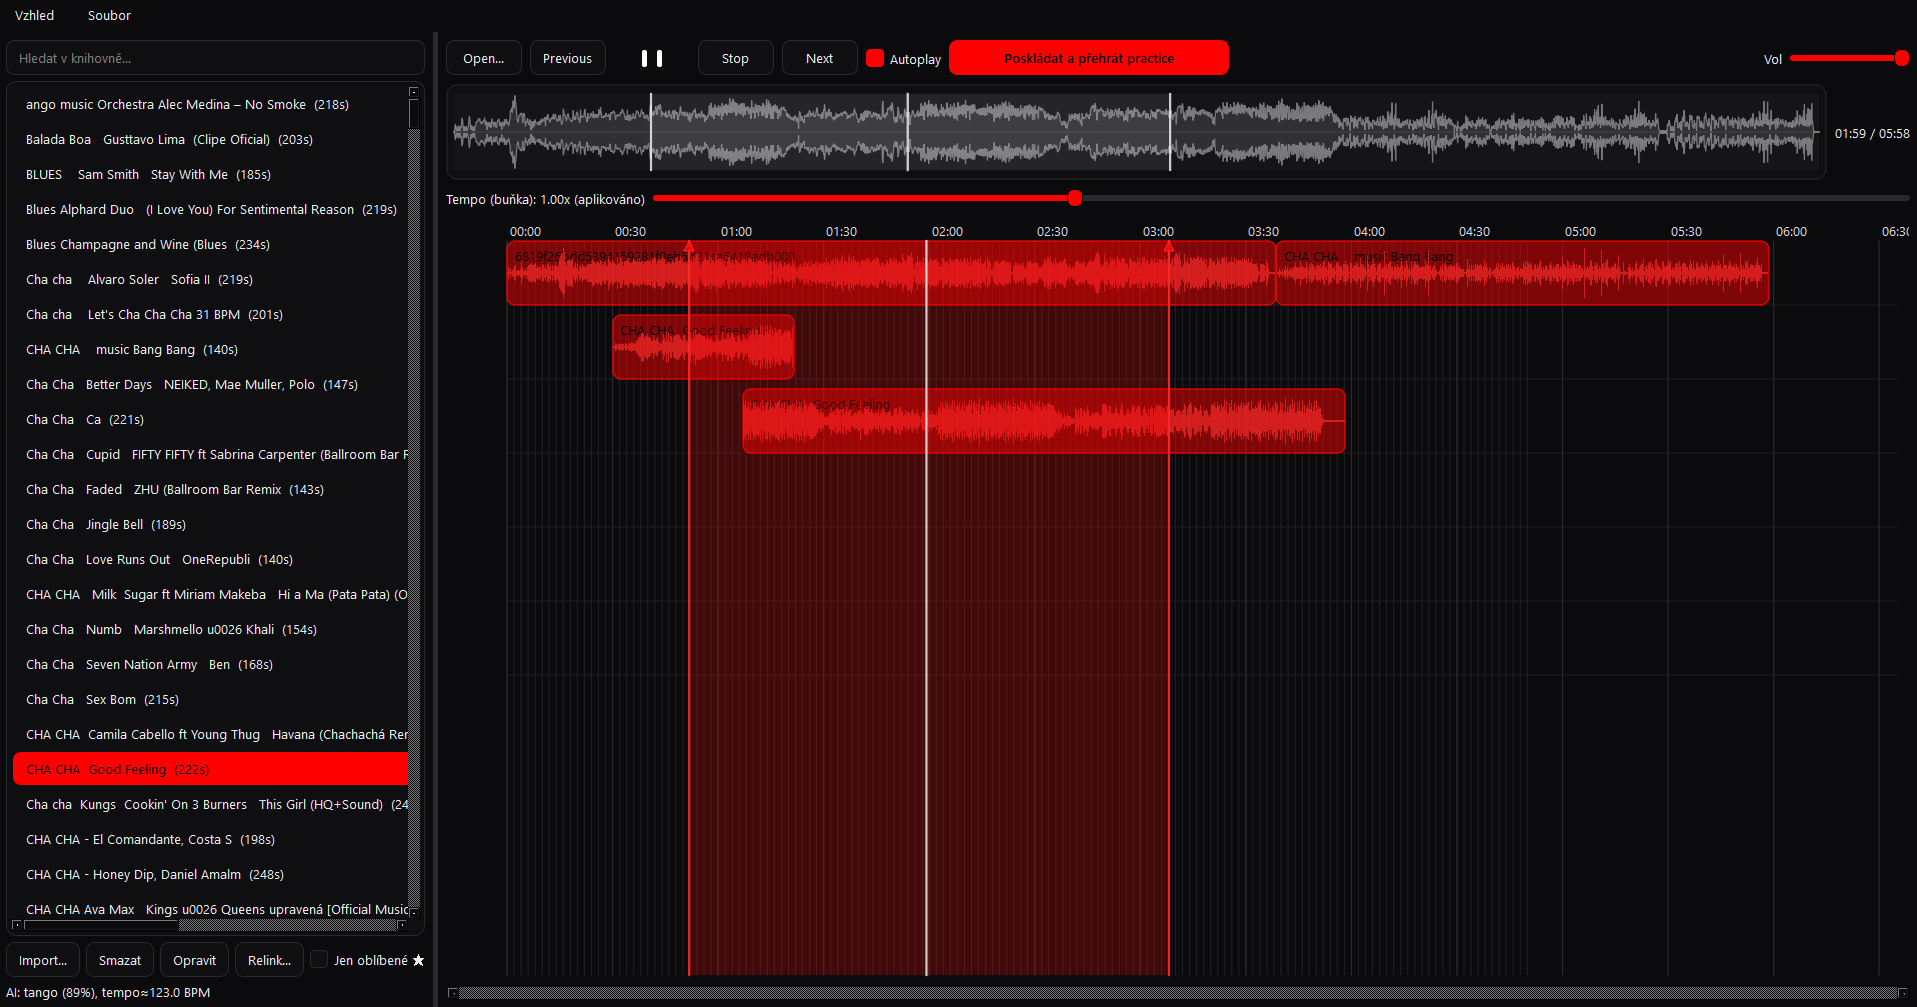
\includegraphics[width=\textwidth]{image/prazmas-main.png}
  \caption{Hlavní okno aplikace \textit{prazmas} s knihovnou skladeb, timeline a editorem buněk během vytváření mixu.}
  \label{fig:prazmas-main}
\end{figure}

\newpage
\section{Architektura aplikace}

Na úrovni architektury je aplikace rozdělena na několik hlavních částí, které spolu komunikují přes jasně definovaná rozhraní. V centru stojí třída \texttt{MainWindow}, která propojuje uživatelské rozhraní s logikou přehrávání a generování mixů. \texttt{MainWindow} vlastní instanci třídy \texttt{AudioPlayer} zodpovědné za nízkoúrovňové přehrávání zvuku, instanci \texttt{TimelineWidget} pro zobrazení průběhu mixu a instanci \texttt{TrackEditorWidget} pro práci s jednotlivými buňkami.

Knihovna skladeb je reprezentována třídou \texttt{Library}, která spravuje databázi dostupných skladeb a poskytuje metody pro jejich import, mazání a opravu záznamů. V grafickém rozhraní je knihovna zobrazena pomocí widgetu \texttt{TrackListWidget}, jenž rozšiřuje standardní seznam Qt o kontextové menu, označování oblíbených skladeb a podporu drag \& drop do editoru. AI modul je zapouzdřen ve třídě \texttt{DanceAI}, která poskytuje jednoduché rozhraní pro odhad tanečního stylu a BPM na základě audio souboru. Celkový návrh tak kombinuje specializované komponenty pro přehrávání, editaci a analýzu zvuku do jednoho uceleného nástroje pro přípravu practice mixů.


\section{Editor buněk a timeline}

Klíčovou částí aplikace je editor buněk, který umožňuje skládat jednotlivé úseky skladeb do výsledného tréninkového mixu. Každý úsek je reprezentován strukturou \texttt{Cell}, jež obsahuje zejména pozici na časové ose (offset v milisekundách), délku po aplikaci tempa, název souboru, název skladby, původní délku v přirozeném tempu a parametry efektů (gain v~dB, délku fade‑in a fade‑out, případně zapnutí echo efektu a jeho parametry). Změna tempa u buňky se neprojevuje pouze vizuálně, ale přepočítává i skutečnou délku úseku tak, aby celkové aranžmá časově odpovídalo zvolenému tempu.

Buňky jsou vykresleny ve více paralelních „lanech“, což umožňuje skládat složitější kombinace skladeb a přehledně odlišit jednotlivé části mixu. Uživatel může buňky uchopit myší a posouvat horizontálně i vertikálně, kopírovat je nebo rozdělit na dvě části v libovolném místě pomocí příkazu \emph{Cut}. Editor podporuje drag \& drop souborů přímo z operačního systému i z panelu knihovny; při přetažení se automaticky vytvoří nová buňka s načteným waveformem. Konkrétní operace nad buňkou (nastavení efektů, smazání, rozdělení v aktuální pozici přehrávací hlavy) jsou dostupné přes kontextové menu vyvolané pravým tlačítkem myši.

Timeline nad editorem zobrazuje průběh celého mixu jako waveform a zároveň slouží k nastavení reprodukčního loopu pomocí dvojice značek A/B. Přehrávací hlava je synchronizována s audio přehrávačem tak, aby se její pohyb v reálném čase shodoval se slyšeným zvukem. Uživatel může kdykoli kliknutím na timeline skočit na jinou pozici, zoomovat časovou osu pomocí kolečka myši nebo nastavit, že se bude přehrávat pouze vybraná část v rámci A/B loopu, což je užitečné při detailním ladění přechodů mezi buňkami.

\section{Generování practice mixů}

Součástí aplikace \textit{prazmas} je průvodce pro automatické generování practice mixů, který má trenérům ušetřit čas při přípravě tréninkových bloků. Při spuštění generování uživatel zadá parametry v dialogu (obr.~\ref{fig:practice-dialog}): 
délku jednoho tance, délku pauzy mezi jednotlivými tanci, volbu typu sekvence (standardní \mbox{STT} nebo latinské \mbox{LAT}) a možnost, zda se má hotový mix uložit do knihovny pro pozdější znovupoužití.

\begin{figure}[h!]
  \centering
  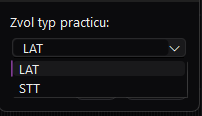
\includegraphics[width=0.5\textwidth]{image/practice-dialog.png}
  \caption{Dialog automatického generování practicu.}
  \label{fig:practice-dialog}
\end{figure}

Typ tance je v aplikaci reprezentován pevně danými skupinami. Pro latinské tance (\mbox{LAT}) se pracuje s pěticí samba, cha‑cha, rumba, paso doble a jive, zatímco standardní skupina (\mbox{STT}) zahrnuje waltz, tango, viennese waltz, slowfox a quickstep. Pro zvolený typ aplikace vytvoří sekvenci tanců v daném pořadí a ke každému tanci se pokouší najít vhodnou skladbu z lokální knihovny, která splňuje požadovanou délku a styl.

Při výběru konkrétní skladby z knihovny se pro každý kandidátní soubor znovu spouští AI modul \texttt{DanceAI}, který analyzuje audio a spočítá pravděpodobnosti příslušnosti k jednotlivým tanečním stylům. Tyto výsledky se nikde trvale neukládají – používají se pouze v daném okamžiku pro rozhodnutí, zda skladba projde filtrem pro aktuálně generovaný tanec. Pokud je pravděpodobnost pro daný styl dostatečně vysoká, skladba je zařazena do mixu; v opačném případě se volí jiná skladba.

Jakmile jsou pro celou sekvenci tanců vybrány odpovídající skladby, aplikace pro každý tanec vytvoří v editoru buněk jednu nebo více buněk o požadované délce a mezi ně vloží pauzy podle zadaného intervalu. Výsledkem je plně připravený practice blok s nastavenými tempy a pauzami, který lze okamžitě přehrát, ručně dále upravit v editoru buněk nebo uložit do knihovny pro pozdější použití na dalších trénincích.

\section{Mixdown a export}

Jakmile je practice mix v editoru hotový, je potřeba převést celé aranžmá do jednoho souboru, který lze přehrát i mimo aplikaci. Tuto funkci zajišťuje mixdown pipeline využívající kombinaci editoru buněk, pomocného modulu \texttt{audio.processing} a externího nástroje FFmpeg. Nejprve \texttt{TrackEditorWidget} spočítá celkovou délku aranžmá a připraví seznam všech buněk včetně jejich offsetu, tempa, efektů a referencí na zdrojové soubory. Následně modul \texttt{audio.processing} postupně skládá jednotlivé úseky do jednoho audio streamu – aplikuje nastavené tempo, gain, fade‑in a fade‑out a případný echo efekt, a to s využitím knihovny pydub.

Pro dekódování vstupních souborů a výslednou konverzi do cílového formátu je použit FFmpeg, který se stará o podporu různých typů vstupních souborů i o správné kódování výstupu. Základním výstupním formátem je nekomprimovaný WAV, aby nedocházelo ke ztrátě kvality při dalších úpravách. Podle zvolených parametrů může aplikace výsledný mix následně překódovat také do ztrátového formátu MP3 nebo bezeztrátového FLAC, což je vhodné pro běžné použití na tréninzích a přenos mezi zařízeními. Uživatel má možnost uložit mix přímo do knihovny aplikace, nebo vybrat libovolné umístění na disku.
\newpage
\section{Testování funkcí aplikace}

Při vývoji aplikace \textit{prazmas} bylo testování zaměřeno hlavně na stabilitu přehrávání, správnou práci s časem a ověření chování editoru při typických scénářích práce trenéra. Testování probíhalo průběžně během vývoje formou manuálních testů na několika projektech, které kombinovaly různé délky skladeb, změny tempa a více buněk na různých lanech. Zvláštní pozornost byla věnována plynulosti přehrávání při posouvání přehrávací hlavy, vypínání a zapínání loopu a přepínání skladeb v režimu \emph{Autoplay}.

Důležitou částí testů bylo ověřit, že změny provedené v editoru buněk se správně promítají do výsledného mixdownu. Testovaly se zejména následující situace: přidávání a mazání buněk, jejich kopírování, rozdělení buňky v různých pozicích, kombinace fade‑in a fade‑out na více na sebe navazujících úsecích a aplikace echo efektu. U každého testu se porovnávala délka a průběh mixu v editoru s výsledným WAV souborem, aby bylo jisté, že časování a použití efektů odpovídá tomu, co uživatel vidí v rozhraní. Samostatně byl ověřován i AI modul: pro sadu předem označených skladeb se kontrolovalo, zda model přiřadí správný dominantní taneční styl a přibližné BPM v očekávaném rozsahu.

\section{Uživatelský manuál}

Tato sekce stručně popisuje typický postup práce s aplikací \textit{prazmas} z pohledu běžného uživatele.

\subsection*{Import skladeb do knihovny}

Uživatel nejprve otevře aplikaci a v levém panelu knihovny použije tlačítko \emph{Import}. V zobrazeném dialogu vybere jednu nebo více audio stop z disku a potvrdí jejich přidání. Aplikace uloží informace o souborech do interní databáze a v seznamu knihovny se zobrazí nové položky s názvem souboru a základními údaji o délce. Pokud jsou některé soubory později přesunuty nebo smazány, lze pomocí tlačítek \emph{Opravit} a \emph{Relink} knihovnu zkontrolovat a chybějící cesty znovu nastavit.
\newpage
\subsection*{Ruční vytvoření practice mixu}

Pro ruční vytvoření practice mixu uživatel přetáhne vybrané skladby z knihovny do editoru buněk v pravé části okna. Každé přetažení vytvoří novou buňku, kterou lze myší posouvat po časové ose, přesouvat na jiný lane a kopírovat. Kontextové menu umožňuje buňku rozdělit na dvě části, upravit hlasitost a nastavit fade‑in nebo fade‑out, případně zapnout echo efekt. Uživatel si tak může poskládat libovolnou kombinaci úseků a přizpůsobit jejich délku a efekty podle potřeby tréninku. 

\subsection*{Automatické generování mixu}

Pokud chce uživatel využít automatické generování practice mixu, otevře příslušný dialog a zadá základní parametry: typ sekvence (standardní STT nebo latinské LAT), délku jednoho tance a délku pauzy mezi tanci. Volitelně může zvolit, zda se má výsledný mix uložit do knihovny. Aplikace následně projde lokální knihovnu skladeb, pro každý tanec vybere vhodné kandidáty a pomocí AI modulu ověří, zda hudba odpovídá požadovanému stylu. Výsledný blok se automaticky naplní do editoru buněk, kde jej lze dále ručně upravovat.


\subsection*{export mixu}

Jakmile je mix hotový, může uživatel projekt exportovat. Pro použití se využije funkce \emph{Export}, která provede mixdown a uloží výsledný soubor jako WAV; podle nastavení může být následně překódován do MP3 nebo FLAC. Exportovaný soubor lze přenést na jiné zařízení nebo použít v běžném přehrávači na tréninku.

\section{Zhodnocení splněných cílů}

V úvodní části práce byly stanoveny cíle, které měla aplikace \textit{prazmas} splnit. V průběhu vývoje se podařilo realizovat všechny klíčové funkce: uživatel může vytvářet practice mixy z~libovolných skladeb v lokální knihovně, pracovat s časovou osou a více buňkami, měnit tempo, aplikovat základní efekty a využít automatické generování sekvencí pro standardní i latinské tance. Implementovaný AI modul dokáže pro každou skladbu odhadnout dominantní taneční styl a přibližné BPM, což usnadňuje kontrolu vhodnosti hudby pro daný typ tréninku. 

Aplikace splňuje i praktické požadavky na použití v tréninkovém prostředí: běží jako samostatný desktopový program bez závislosti na internetu, podporuje ovládání pomocí multimediálních kláves a tlačítek na bezdrátových sluchátkách a umožňuje export hotových mixů do běžných formátů. Některé oblasti zůstávají otevřené pro budoucí rozšíření, například pokročilejší správa projektů, sdílení presetů practice bloků mezi uživateli nebo integrace s online databázemi hudby. Z hlediska původně vytyčených cílových požadavků však lze projekt považovat za úspěšně realizovaný funkční prototyp, který je připravený k reálnému nasazení na trénincích.


\chapter*{Závěr}
\addcontentsline{toc}{chapter}{Závěr}

Cílem práce bylo navrhnout a vytvořit desktopovou aplikaci \textit{prazmas}, která zjednoduší trenérům párových tanců přípravu a přehrávání tréninkových hudebních mixů. Aplikace měla nabídnout knihovnu skladeb, editor s časovou osou, náhodné generování practice bloků, AI analýzu tanečních stylů a export do běžných audio formátů – vše v jednom offline nástroji bez závislosti na internetu.

Všechny stanovené cíle byly splněny: uživatel může importovat skladby do lokální knihovny, skládat je do editoru buněk s podporou více lanech, měnit tempo jednotlivých úseků, aplikovat efekty (fade-in/out, gain, echo) a nastavovat loop. Automatické generování practice mixů pro standardní (STT) i latinské (LAT) tance využívá AI modul k ověření stylové shody skladeb a vytváří plynulé sekvence s nastavitelnými pauzami. Výsledné aranžmá lze exportovat jako WAV, MP3 nebo FLAC a ovládat i přes multimediální klávesy či sluchátka.

Aplikace je postavena na Pythonu s PyQt6, pydubem a FFmpegem, což zajišťuje stabilitu i multiplatformnost. Testování prokázalo spolehlivost při reálných scénářích – od krátkých loopů po delší practice bloky.

Do budoucna lze rozšířit například pokročilou správu projektů s verzováním, sdílení presetů practice mezi uživateli, integraci s online hudebními službami nebo vylepšení AI o rozpoznávání struktury skladby (úvod, refrén). Přesto je \textit{prazmas} plně použitelným prototypem připraveným k nasazení na trénincích.


% ---------- LITERATURA ----------
\begin{thebibliography}{99}

\bibitem{pyqt6}
Riverbank Computing, ``PyQt6 Reference Guide'', 
\url{https://www.riverbankcomputing.com/static/Docs/PyQt6/}, 
cit. 4.~1.~2026.

\bibitem{pydub}
Jiaaro, ``pydub - Simple audio libraries for Python'', 
\url{https://github.com/jiaaro/pydub}, 
cit. 4.~1.~2026.

\bibitem{ffmpeg}
FFmpeg Project, ``FFmpeg Documentation'', 
\url{https://ffmpeg.org/documentation.html}, 
cit. 4.~1.~2026.

\bibitem{python312}
Python Software Foundation, ``Python 3.12 Documentation'', 
\url{https://docs.python.org/3.12/}, 
cit. 4.~1.~2026.

\bibitem{librosa}
McFee, B. et al., ``librosa: Audio and Music Signal Analysis in Python'', 
\url{https://librosa.org/doc/latest/index.html}, 
cit. 4.~1.~2026.

\bibitem{scipy}
Virtanen, P. et al., ``SciPy 1.0: Fundamental Algorithms for Scientific Computing in Python'', 
\url{https://docs.scipy.org/doc/scipy/reference/}, 
2018.

\bibitem{pyqt6-designer}
The Qt Company, ``Qt Designer Manual'', 
\url{https://doc.qt.io/qt-6/qtdesigner-manual.html}, 
cit. 4.~1.~2026.

\bibitem{qt-audio}
The Qt Company, ``Qt Multimedia Overview'', 
\url{https://doc.qt.io/qt-6/qtmultimedia-index.html}, 
cit. 4.~1.~2026.

\end{thebibliography}

\end{document}
